\documentclass[11pt]{article}
%\usepackage[firstpage]{draftwatermark}
\usepackage{times}
\usepackage{pdfpages}
\usepackage{fullpage}
\usepackage{url}
\usepackage{hyperref}
\usepackage{fancyhdr}
\usepackage{graphicx}
\usepackage{tabularx}
\usepackage{enumitem}
\usepackage{indentfirst}
\usepackage{subcaption}
\usepackage{units}
\usepackage{bm}

\usepackage{./math_bbing}


% Highlighting
\usepackage{color,soul}
\DeclareRobustCommand{\hlr}[1]{{\sethlcolor{red}\hl{#1}}}
\DeclareRobustCommand{\hlg}[1]{{\sethlcolor{green}\hl{#1}}}
\DeclareRobustCommand{\hlb}[1]{{\sethlcolor{blue}\hl{#1}}}
\DeclareRobustCommand{\hly}[1]{{\sethlcolor{yellow}\hl{#1}}}

\setcounter{secnumdepth}{4}
\graphicspath{{images/}}
\pagestyle{fancy}

% Conditional for notes
\newif\ifnotes
\notesfalse


\newcommand{\doctitle}{USV Plugins, Theory of Operation}

\newcommand{\docnumber}{\doctitle}

\addtolength{\headheight}{2em}
\addtolength{\headsep}{1.5em}
\lhead{\docnumber}
\rhead{}

\newcommand{\capt}[1]{\caption{\small \em #1}}

\cfoot{\small Brian Bingham \today \\ \thepage}
\renewcommand{\footrulewidth}{0.4pt}

\newenvironment{xitemize}{\begin{itemize}\addtolength{\itemsep}{-0.75em}}{\end{itemize}}
\newenvironment{tasklist}{\begin{enumerate}[label=\textbf{\thesubsubsection-\arabic*},ref=\thesubsubsection-\arabic*,leftmargin=*]}{\end{enumerate}}
\newcommand\todo[1]{{\bf TODO: #1}}
\setcounter{tocdepth}{2}
\setcounter{secnumdepth}{4}

\makeatletter
\newcommand*{\compress}{\@minipagetrue}
\makeatother

%\renewcommand{\chaptername}{Volume}
%\renewcommand{\thesection}{\Roman{section}}
%\renewcommand{\thesubsection}{\Roman{section}-\Alph{subsection}}

\begin{document}
% List of new commands
% bbing 06-11-98

%\newcommand{\spacing}[1]{\renewcommand{\baselinestretch}{#1} \normalsize}

% Degree symbol within text
\newcommand{\degrees}{$^{\circ}$}
\newcommand{\CRlb}{Cram\'{e}r Rao }

\newcommand{\btab}{\begin{tabular}}
\newcommand{\etab}{\end{tabular}}

\newcommand{\bfig}{\begin{figure}}
\newcommand{\efig}{\end{figure}}

\newcommand{\beqn}{\begin{equation}}
\newcommand{\eeqn}{\end{equation}}
\newcommand{\bdm}{\begin{displaymath}}
\newcommand{\edm}{\end{displaymath}}

\newcommand{\bearray}{\begin{eqnarray}}
\newcommand{\eearray}{\end{eqnarray}}
\newcommand{\Bearray}{\begin{eqnarray}}
\newcommand{\Eearray}{\end{eqnarray}}

\newcommand{\bgat}{\begin{gather}}
\newcommand{\egat}{\end{gather}}

\newcommand{\Htwo}{$\mathcal{H}_2$\ }
\newcommand{\Hinf}{$\mathcal{H}_{\infty}$\ }

%\newcommand{\V}[1]{\mathbf{#1}}
\newcommand{\plusminus}{{\textstyle \frac{+}{-}}}

\newcommand{\TM}{$^{TM}$}

% Definitions  %from homero!
%
%\newcommand{\mtitle}[1]{\begin{center} {\huge \bf{#1}}\end{center}}
\newcommand{\lb}{\linebreak}
\newcommand{\xaxis}{\mbox{$x$-axis}}
\newcommand{\yaxis}{\mbox{$y$-axis}}
\newcommand{\zaxis}{\mbox{$z$-axis}}
\newcommand{\bc}{\begin{center}}
\newcommand{\ec}{\end{center}}
%\newcommand{\be}{\begin{equation}}
%\newcommand{\ee}{\end{equation}}
\newcommand{\bd}{\begin{displaymath}}
\newcommand{\ed}{\end{displaymath}}
\newcommand{\bi}{\begin{itemize}}
\newcommand{\ei}{\end{itemize}}
%\newcommand{\bt}{\begin{tabular}}
%\newcommand{\et}{\end{tabular}}
\newcommand{\ba}{\begin{array}}
\newcommand{\ea}{\end{array}}
\newcommand{\baa}[2]{\begin{array}[t]{cc}
\left[#1\right.\!\!&\!\!\left.#2\right]\end{array}} 
\newcommand{\bea}{\begin{eqnarray}}
\newcommand{\eea}{\end{eqnarray}}
\newcommand{\bsea}{\begin{subeqnarray}}
\newcommand{\esea}{\end{subeqnarray}}
\newcommand{\degr}{\mbox{$^{\circ}$}}
\newcommand{\jw}{j\omega}
\newcommand{\dw}{\mbox{\rm d}\omega}
\newcommand{\dx}[1]{\,\mbox{\rm d}#1}
\newcommand{\til}{^{\sim}}
\newcommand{\abcd}[4]{\left[\begin{array}{c|c}#1&#2\\ \hline #3&#4 
\end{array}\right]}
\newcommand{\etal}{{\em et al.}}
\newcommand{\etc}{{\em etc.}}
\newcommand{\eg}{{\em e.g., }}
\newcommand{\ie}{{\em i.e., }}
\newcommand{\eqnref}[1]{Equation~(\ref{#1})}
\newcommand{\eqrefa}[1]{Eq'n~(\ref{#1})}
\newcommand{\eqrefb}[1]{(\ref{#1})}
\newcommand{\expec}[1]{\left\langle #1 \right\rangle}
\newcommand{\pder}[2]{\frac{\partial #1}{\partial #2}}
\newcommand{\half}{{\textstyle \frac{1}{2}}}
\newcommand{\msp}{\mbox{\hspace{.5in}}}
\newcommand{\ub}[2]{\underbrace{#1}_{#2}}
\newcommand{\eqn}[1]{Eq.~\ref{eq:#1}}
%
%\newenvironment{proof}{\par\noindent{\bf Proof: }}{\hfill $\Box$}
%\newenvironment{remark}{{\bf Remark: }}{}
%
\def\sinc{\mathop{\rm sinc}\nolimits}
%
\newcommand{\vdashes}[2]
   {{\vfuzz #1 \vbox to 0pt{\vskip -#2
   \vbox{\xleaders\vbox{\vskip 1pt\hfuzz 1pt\hbox to 0pt{\vrule height 4pt
   depth 0pt}\vskip 1pt}\vskip #1}}}}


\newcommand{\bmat}[1]{\left[ \begin{array}{#1}}
\newcommand{\emat}{\end{array} \right]}
%\newcommand{\bvec}{\left( \begin{array}{c}}
\newcommand{\evec}{\end{array} \right)}

  
% Stolen from Austratlian Center for Field Robotics
% Thanks Alex!
% bbing 24.02.03

% references to figurs and equations
\newcommand{\fref}[1] {Figure~\ref{#1}}
\newcommand{\eref}[1] {~(\ref{#1})}

% general global definitions
\newcommand{\Def}{\ {\buildrel \triangle\over =}\ }
%\newcommand{\beq} {\begin{equation}}
%\newcommand{\eeq} {\end{equation}}
%\newcommand{\beqn} {\begin{eqnarray}}
%\newcommand{\eeqn} {\end{eqnarray}}
%\newcommand{\E}[1] {\mbox{$ {\rm E} \{ #1 \}$ }}
\newcommand{\Es}[2] {\mbox{$ {\rm E}^{#1} \{ #2 \}$ }}
\newcommand{\Set}[1] {\mbox{$ \{ #1 \} $ }}
\newcommand{\Cal}[1] {\mbox{$ {\cal #1 } $}}
\newcommand{\PR}[1]  {\mbox{$ P(#1) $}}
\newcommand{\Pri}[2]  {\mbox{$ P_{#1}(#2) $}}
\newcommand{\PRi}[2]  {\mbox{$ P_{#1}(#2) $}}
\newcommand{\Pris}[3]  {\mbox{$ P_{#1}^{#2}(#3) $}}
\newcommand{\like}[1]  {\mbox{$ \Lambda(\bf #1) $}}
\newcommand{\likei}[2]  {\mbox{$ \Lambda_{#2}(\bf #1) $}}
\newcommand{\LL}[1]  {\mbox{$ l(#1) $}} % loglikelihood
\newcommand{\LLi}[2]  {\mbox{$ l_{#1}(#2) $}} %loglikelihood
\newcommand{\EN}[1]  {\mbox{$ H(#1) $}} % entropy
\newcommand{\ENi}[2]  {\mbox{$ H_{#1}(#2) $}} % entropy
\newcommand{\mEN}[1]  {\mbox{$ \overline{H}(#1) $}} % mean entropy
\newcommand{\MI}[1]  {\mbox{$ I(#1) $}}  %mutual information
\newcommand{\est}[1]  {\mbox{$\hat{\bf #1}$}}
\newcommand{\estk}[2]  {\mbox{$\hat{\bf #1}(#2)$}}
\newcommand{\D}[1]    {\mbox{${\rm d} {#1}$}}
\newcommand{\mean}[1] {\mbox{$\overline{ #1}$}}
\newcommand{\Det}[1] {\mbox{$\mid {#1} \mid $}}
\newcommand{\One}      {\mbox{${\bf 1}$}}
\newcommand{\Zero}      {\mbox{${\bf 0}$}}
\newcommand{\grad}[1] {\mbox{${\bf\nabla} #1$}}
\newcommand{\J}[3] {\mbox{${\bf\nabla}{\bf #1}_{\bf #2}(#3)$}}
\newcommand{\Jt}[3] {\mbox{${\bf\nabla}^T{\bf #1}_{\bf #2}(#3)$}}
\newcommand{\pdf}{{\it pdf\ }}
\newcommand{\dxt}[2]  {\mbox{$\dot{\bf #1}( #2)$}}
% defining different types of vectors
% first those with no time subscripts
\newcommand{\V}[1] {\mbox{${\bf #1}$}}
\newcommand{\Vt}[1] {\mbox{${\bf #1}^T$}}
\newcommand{\Vin}[1] {\mbox{${\bf #1}^{-1}$}}
\newcommand{\Vgin}[1] {\mbox{${\bf #1}^{\dagger}$}}
\newcommand{\Vi}[2] {\mbox{${\bf #1}_{#2}$}}
\newcommand{\Vs}[2] {\mbox{${\bf #1}^{#2}$}}
\newcommand{\Vis}[3] {\mbox{${\bf #1}_{#2}^{#3}$}}
\newcommand{\Vit}[2] {\mbox{${\bf #1}_{#2}^T$}}
\newcommand{\Vini}[2] {\mbox{${\bf #1}_{#2}^{-1}$}}
\newcommand{\Vgini}[2] {\mbox{${\bf #1}^{\dagger}$}}

% next those with time subscript k (very common)
\newcommand{\Vk}[1] {\mbox{${\bf #1}(k)$}}
\newcommand{\Vkt}[1] {\mbox{${\bf #1}^T(k)$}}
\newcommand{\Vkin}[1] {\mbox{${\bf #1}^{-1}(k)$}}
\newcommand{\Vkgin}[1] {\mbox{${\bf #1}^{\dagger}(k)$}}
\newcommand{\Vki}[2] {\mbox{${\bf #1}_{#2}(k)$}}
\newcommand{\Vks}[2] {\mbox{${\bf #1}^{#2}(k)$}}
\newcommand{\Vkis}[3] {\mbox{${\bf #1}_{#2}^{#3}(k)$}}
\newcommand{\Vkit}[2] {\mbox{${\bf #1}_{#2}^T(k)$}}
\newcommand{\Vkini}[2] {\mbox{${\bf #1}_{#2}^{-1}(k)$}}
\newcommand{\Vkgini}[2] {\mbox{${\bf #1}^{\dagger}_{#2}(k)$}}
\newcommand{\tVk}[1] {\mbox{$\tilde{\bf #1}(k)$}}
\newcommand{\tVki}[2] {\mbox{$\tilde{\bf #1}_{#2}(k)$}}

% now those with general purpose time subscripts
%\newcommand{\Vec}[2] {\mbox{${\bf #1}(#2)$}}
\newcommand{\Vect}[2] {\mbox{${\bf #1}^T(#2)$}}
\newcommand{\Vecin}[2] {\mbox{${\bf #1}^{-1}(#2)$}}
\newcommand{\Veci}[3] {\mbox{${\bf #1}_{#2}(#3)$}}
\newcommand{\Vecit}[3] {\mbox{${\bf #1}_{#2}^T(#3)$}}
\newcommand{\Vecini}[3] {\mbox{${\bf #1}_{#2}^{-1}(#3)$}}
\newcommand{\Vecgin}[2] {\mbox{${\bf #1}^{\dagger}(#2)$}}
\newcommand{\Vecgini}[3] {\mbox{${\bf #1}^{\dagger}_{#2}(#3)$}}

% special symbols used very commonly
% state estimates of different sorts
\newcommand{\x}[2] {\mbox{$\hat{\bf x}( #1 \mid #2)$}}
\newcommand{\ix}[3] {\mbox{$\hat{\bf x}_{#1}( #2 \mid #3)$}}
\newcommand{\tx}[2] {\mbox{$\tilde{\bf x}( #1 \mid #2 )$}}
\newcommand{\txi}[3] {\mbox{$\tilde{\bf x}_{#1}( #2 \mid #3 )$}}
\newcommand{\z}[2] {\mbox{$\hat{\bf z}( #1 \mid #2)$}}
\newcommand{\tz}[2] {\mbox{$\tilde{\bf z}( #1 \mid #2)$}}
\newcommand{\tzt}[2] {\mbox{$\tilde{\bf z}^T( #1 \mid #2)$}}
\newcommand{\zi}[3] {\mbox{$\hat{\bf z}_{#1}( #2 \mid #3)$}}
\newcommand{\di}[3] {\mbox{$\hat{\bf \delta}_{#1}( #2 \mid #3)$}}

% variances of different sorts
\newcommand{\var}[2] {\mbox{${\bf P}( #1 \mid #2)$}}
\newcommand{\varin}[2] {\mbox{${\bf P}^{-1}( #1 \mid #2)$}}
\newcommand{\tvar}[2] {\mbox{$\tilde{\bf P}( #1 \mid #2)$}}
\newcommand{\tvarin}[2] {\mbox{$\tilde{\bf P}^{-1}( #1 \mid #2)$}}
\newcommand{\vari}[3] {\mbox{${\bf P}_{#1}( #2 \mid #3)$}}
\newcommand{\varini}[3] {\mbox{${\bf P}^{-1}_{#1}( #2 \mid #3)$}}
\newcommand{\tvari}[3] {\mbox{$\tilde{\bf P}_{#1}( #2 \mid #3)$}}
\newcommand{\tvarini}[3] {\mbox{$\tilde{\bf P}^{-1}_{#1}( #2 \mid #3)$}}

% information states and variances
\newcommand{\y}[2] {\mbox{$\hat{\bf y}( #1 \mid #2)$}}
\newcommand{\ty}[2] {\mbox{$\tilde{\bf y}( #1 \mid #2)$}}
\newcommand{\yi}[3] {\mbox{$\hat{\bf y}_{#1}( #2 \mid #3)$}}
\newcommand{\tyi}[3] {\mbox{$\tilde{\bf y}_{#1}( #2 \mid #3)$}}
\newcommand{\Y}[2] {\mbox{${\bf Y}( #1 \mid #2)$}}
\newcommand{\Yin}[2] {\mbox{${\bf Y}^{-1}( #1 \mid #2)$}}
\newcommand{\tY}[2] {\mbox{$\tilde{\bf Y}( #1 \mid #2)$}}
\newcommand{\Yi}[3] {\mbox{${\bf Y}_{#1}( #2 \mid #3)$}}
\newcommand{\Yini}[3] {\mbox{${\bf Y}_{#1}^{-1}( #2 \mid #3)$}}
\newcommand{\tYi}[3] {\mbox{$\tilde{\bf Y}_{#1}( #2 \mid #3)$}}
\newcommand{\info}[1] {\mbox{${\bf i}( #1)$}}
\newcommand{\Info}[1] {\mbox{${\bf I}( #1)$}}
\newcommand{\infoi}[2] {\mbox{${\bf i}_{#1}( #2)$}}
\newcommand{\infois}[3] {\mbox{${\bf i}_{#1}^{#2}(#3)$}}
\newcommand{\Infoi}[2] {\mbox{${\bf I}_{#1}( #2)$}}
\newcommand{\tInfoi}[2] {\mbox{$\tilde{\bf I}_{#1}( #2)$}}
\newcommand{\Infoini}[2] {\mbox{${\bf I}^{\dagger}_{#1}( #2)$}}
\newcommand{\Prop}[2] {\mbox{${\bf L}( #1 \mid #2)$}}
\newcommand{\Propi}[3] {\mbox{${\bf L}_{#1}( #2 \mid #3)$}}
\newcommand{\Z}[2] {\mbox{${\cal Z}^{#1}_{#2}$}}

% spurious ones
\newcommand{\maybe}{\ {\buildrel ?\over =}\ } %chapter 4
\newcommand{\svd} {\mbox{$\dagger$}} % chapter 4
\newcommand{\dnoise} {\mbox{$\delta d$}} % chapter 6 and 7
\newcommand{\unoise} {\mbox{$\delta u$}} % chapter 6
\newcommand{\ns}[1] {\mbox{$ #1$}} % chapter 6
\newcommand{\vs} {\vspace{0.17in}}
\newcommand{\svs} {\vspace{0.17cm}}
\newcommand{\vsf} {\vspace{0.4in}}
\newcommand{\vsff} {\vspace{1in}}
\newcommand{\veqns} {\vspace{-0.15in}}
\newcommand{\veqn} {\vspace{-0.12in}}
\newcommand{\sveqn} {\vspace{-0.06in}}
%\newcommand{\bc}{\begin{center}}
%\newcommand{\ec}{\end{center}}
%\newcommand{\bi}{\begin{itemize}}
%\newcommand{\ei}{\end{itemize}}
%\newcommand{\be}{\begin{enumerate}}
%\newcommand{\ee}{\end{enumerate}}
\newcommand{\Quote}{\parbox[t]{12.5cm}}
\newtheorem{example}{Example}

\newpage
% Title Page
\setcounter{page}{1}
\begin{center}
{\huge \doctitle}
\end{center}


\section{Overview}
The rigid body dynamics implemented in Gazebo are augmented with environmental forces to simulate an unmanned surface vessel via a set of Gazebo plugins.  These plugins simulate the effects of
\begin{itemize}
\item Dynamics
  \begin{itemize}
  \item Maneuvering - added mass, drag, etc.
  \item Wave field - motion of the water surface
  \end{itemize}
\item Thrust - vehicle propulsion
\item Wind - windage.
  \end{itemize}

This document is a high-level description of the implementation, but not a full documentation of the models and techniques used.  The code itself is the ultimate documentation; comments have been included in the source to allow for users to adapt and extend these simple techniques for their own purposes.

\section{Maneuvering Model and Waves}
The influence of both maneuvering and wave forces on the motion of the USV is implemented as a single model plugin for Gazebo.  Currently there is only one implementation, but other implementations, with varying fidelity, could be developed in the future.

\subsection{usv gazebo dynamics plugin}

\subsubsection{Maneuvering Model}
The plugin implements a portion of the nonlinear maneuvering equations from \cite{fossen11handbook}, 
\beqn
\underbrace{\bm{M}_{RB}\dot{\bm{\nu}}+\bm{C}_{RB}(\bm{\nu})\bm{\nu}}_\text{rigid-body forces} +
\underbrace{\bm{M}_A\dot{\bm{\nu}}_r + \bm{C}_A(\bm{\nu}_r)\bm{\nu}_r + 
\bm{D}(\bm{\nu}_r)\bm{\nu}_r}_\text{hydrodynamic forces}
= \bm{\tau}+\bm{\tau}_{wind}+\bm{\tau}_{waves}
\label{e:fossenmodel}
\eeqn
where the state vector $\bm{\nu}=[u,v,r]^T$ includes the velocities $u$, $v$ and $r$ are in the surge, sway and yaw directions respectively and  $\bm{\nu}_r$ is the velocity vector relative to an irrotational water current $\bm{\nu}_c$, i.e., $\bm{\nu}=\bm{\nu}_r+\bm{\nu}_c$.
The \emph{rigid-body forces} components are simulated via the Gazebo physics engine, while the \emph{hydrodynamic forces} are determined via the plugin.


The six DOF maneuvering model is specified by the following matrices. The added mass matrix expressed as 
\beqn
\bm{M}_{A}= \left[ 
\begin{array}{cccccc}
-X_{\dot{u}} & 0 & 0 &0 &0 &0 \\
0 & -Y_{\dot{v}} & 0 &0 &0 &0 \\
0 & 0  &0.1 &0 &0 &0 \\
0 &0 &0 &0.1 &0 &0 \\
0 &0 &0 &0 &0.1 &0 \\
0 &0 &0 &0 & 0 & -N_{\dot{r}} 
\end{array} \right].
\eeqn
The Coriolis-centripetal matrix for the added mass expressed as 
\beqn
\bm{C}_{A}(\bm{\nu}_r)= \left[ 
\begin{array}{cccccc}
0 &0 &0 &0 & 0 & Y_{\dot{v}}v_r+Y_{\dot{r}}r \\
0 &0 &0 &0 & 0 & -X_{\dot{u}}u_r\\
0 &0 &0 &0 &0 &0 \\
0 &0 &0 &0 &0 &0 \\
0 &0 &0 &0 &0 &0 \\
0 &0 &0 & -Y_{\dot{v}}v_r - Y_{\dot{r}}r& X_{\dot{u}}u_r & 0 
\end{array} \right].
\eeqn.
It is worth noting that $\bm{C}_A$ includes the nonlinear Munk moment (see \cite{fossen11handbook} p.121).  Following \cite{fossen11handbook} the SNAME notation for the hydrodynamic derivatives.  Currently these terms are neglected in the model for simplicity and because of the challenges in estimating and verifying the pertinent parameters.

The linear and quadratic drag terms
\beqn
\bm{D}(\bm{\nu}_r)= \left[ 
\begin{array}{cccccc}
X_u + X_{u|u|}|u| & 0 & 0 &0 &0 &0\\
0 & Y_v + Y_{v|v|}|v| &0  &0 &0 &0\\
0 &0 &Z_w  &0 &0 &0 \\
0 &0 &0 &K_p  &0 &0 \\
0 &0 &0 &0 &M_q &0 \\
0 &0 &0 &0 &0 & N_r+N_{r|r|}|r|
\end{array} \right].
\eeqn
which neglects coupleing between sway and yaw.


\subsubsection{Wave Forcing}

Gerstner waves with three components \cite{tessendorf99simulating}.  Each of the component waves is user-specified by an amplitude, period and direction.  Deep water dispersion is used in simulating the wave behaviors.

To determine the influence of the wave field on the vessel, the vessel footprint is decomposed into a simple grid, with points at each corner of the vessel.  The vertical displacement is calculated for each of these points.  Using the vessel's position and attitude, the buoyancy force at each location is determined and then applied at that grid point.


\section{Thrust}
The external force and torque from the vessel propulsion is implemented in a standalone plugin to allow for independent extension to higher-fidelity thrust configurations and models.

\subsection{usv gazebo thrust plugin}
The plugin subscribes the \verb+cmd_drive+ topic to receive messages of type UsvDrive (defined in the \verb+usv_msgs+ package).  These message specify left and right thrust commands where the commands are scaled from $\{-1.0-1.0\}$. 

To emulate the thruster behavior, the commands are mapped to a thrust force applied to the model.  Two possible mappings are currently available.  Users select which mapping using the \verb+mappingType+ SDF tag.

The axial force is applied at a point vertically separated from the CG as specified by the \texttt{thrustOffsetZ} parameter.  This results in coupling between the forward thrust and the vehicle pitch.

\subsubsection{0: Linear thruster map}
The command values (-1.0 to 1.0) are scaled linearly to the \texttt{maxForceFwd} and \texttt{maxForceRev} SDF parameters.  A total forward thrust is caculated as the sum.  A total torque is calculated assuming the two thrust forces are applied at opposite ends of the \texttt{boatWidth} parameter.

\subsubsection{1: GLF thruster map}

In this mode two generalized logistic functions (GLFs) are used to convert commands to thrust force.  One set of GLF parameters are used for positive commands (0 to 1.0) and a second set of parameters are used for negative commands (-1 to 0).  The form of the GLF used is
\begin{equation}
  T = A + \frac{K-A}{\left(C+\exp(-B(x-M))\right)^{1/\nu}}
\end{equation}
where $T$ is the thrust force in Newtons, $x$ is the command and the remaining variables are the GLF parameters.  To identify the GLF parameters, the data from 
\cite{sarda17station} was used---Figure\ref{f:sarda}.  The Python script for accomplishing this is include in the \verb+usv_gazebo_plugins+ repository in the \verb+thrust_curve_fit+ directory.

\begin{figure}[h]
  \centering
  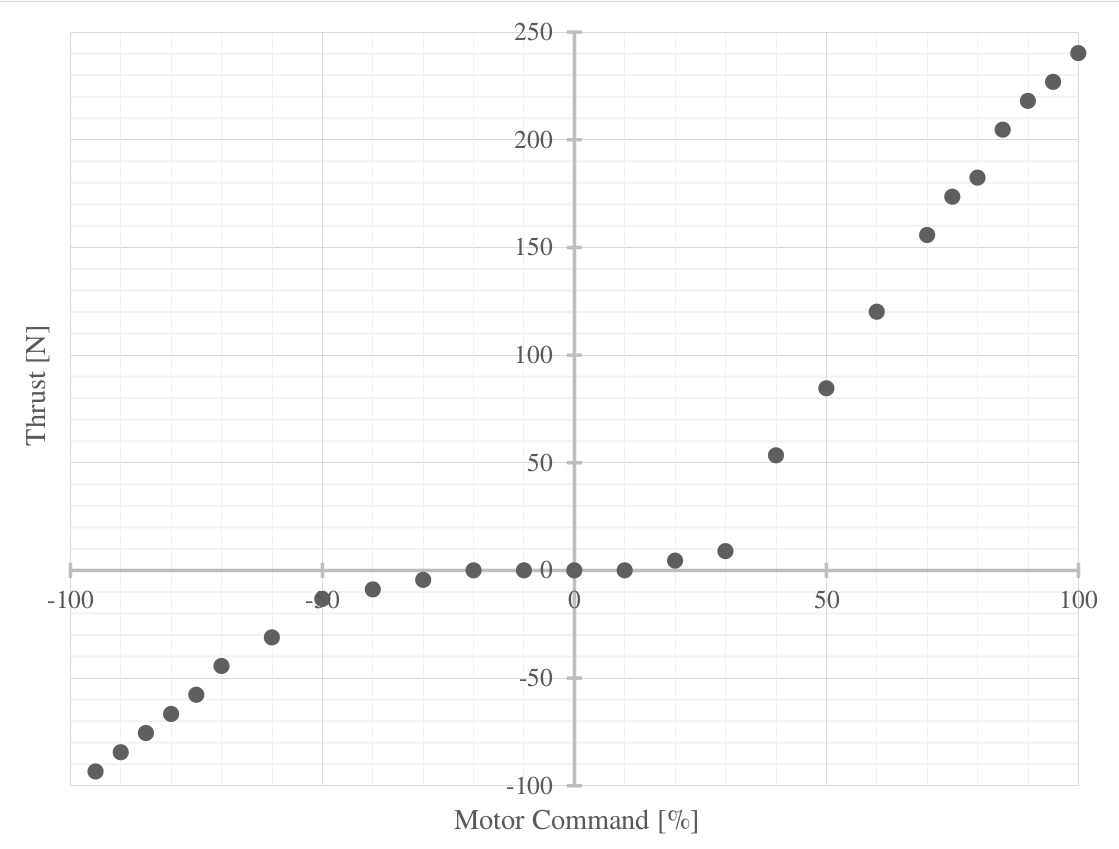
\includegraphics[width=0.6\textwidth]{images/sarda_tcurve.png}
  \caption{Empirical thrust performance data from \cite{sarda17station}.}
  \label{f:sarda}
\end{figure}

The data was fit with two separate GLF functions using the \verb+scipy.optimize.fmin+ optimization routine to minimize the squared error.  The results are shown in Figure\ref{f:fit}.

\begin{figure}[h]
  \centering
  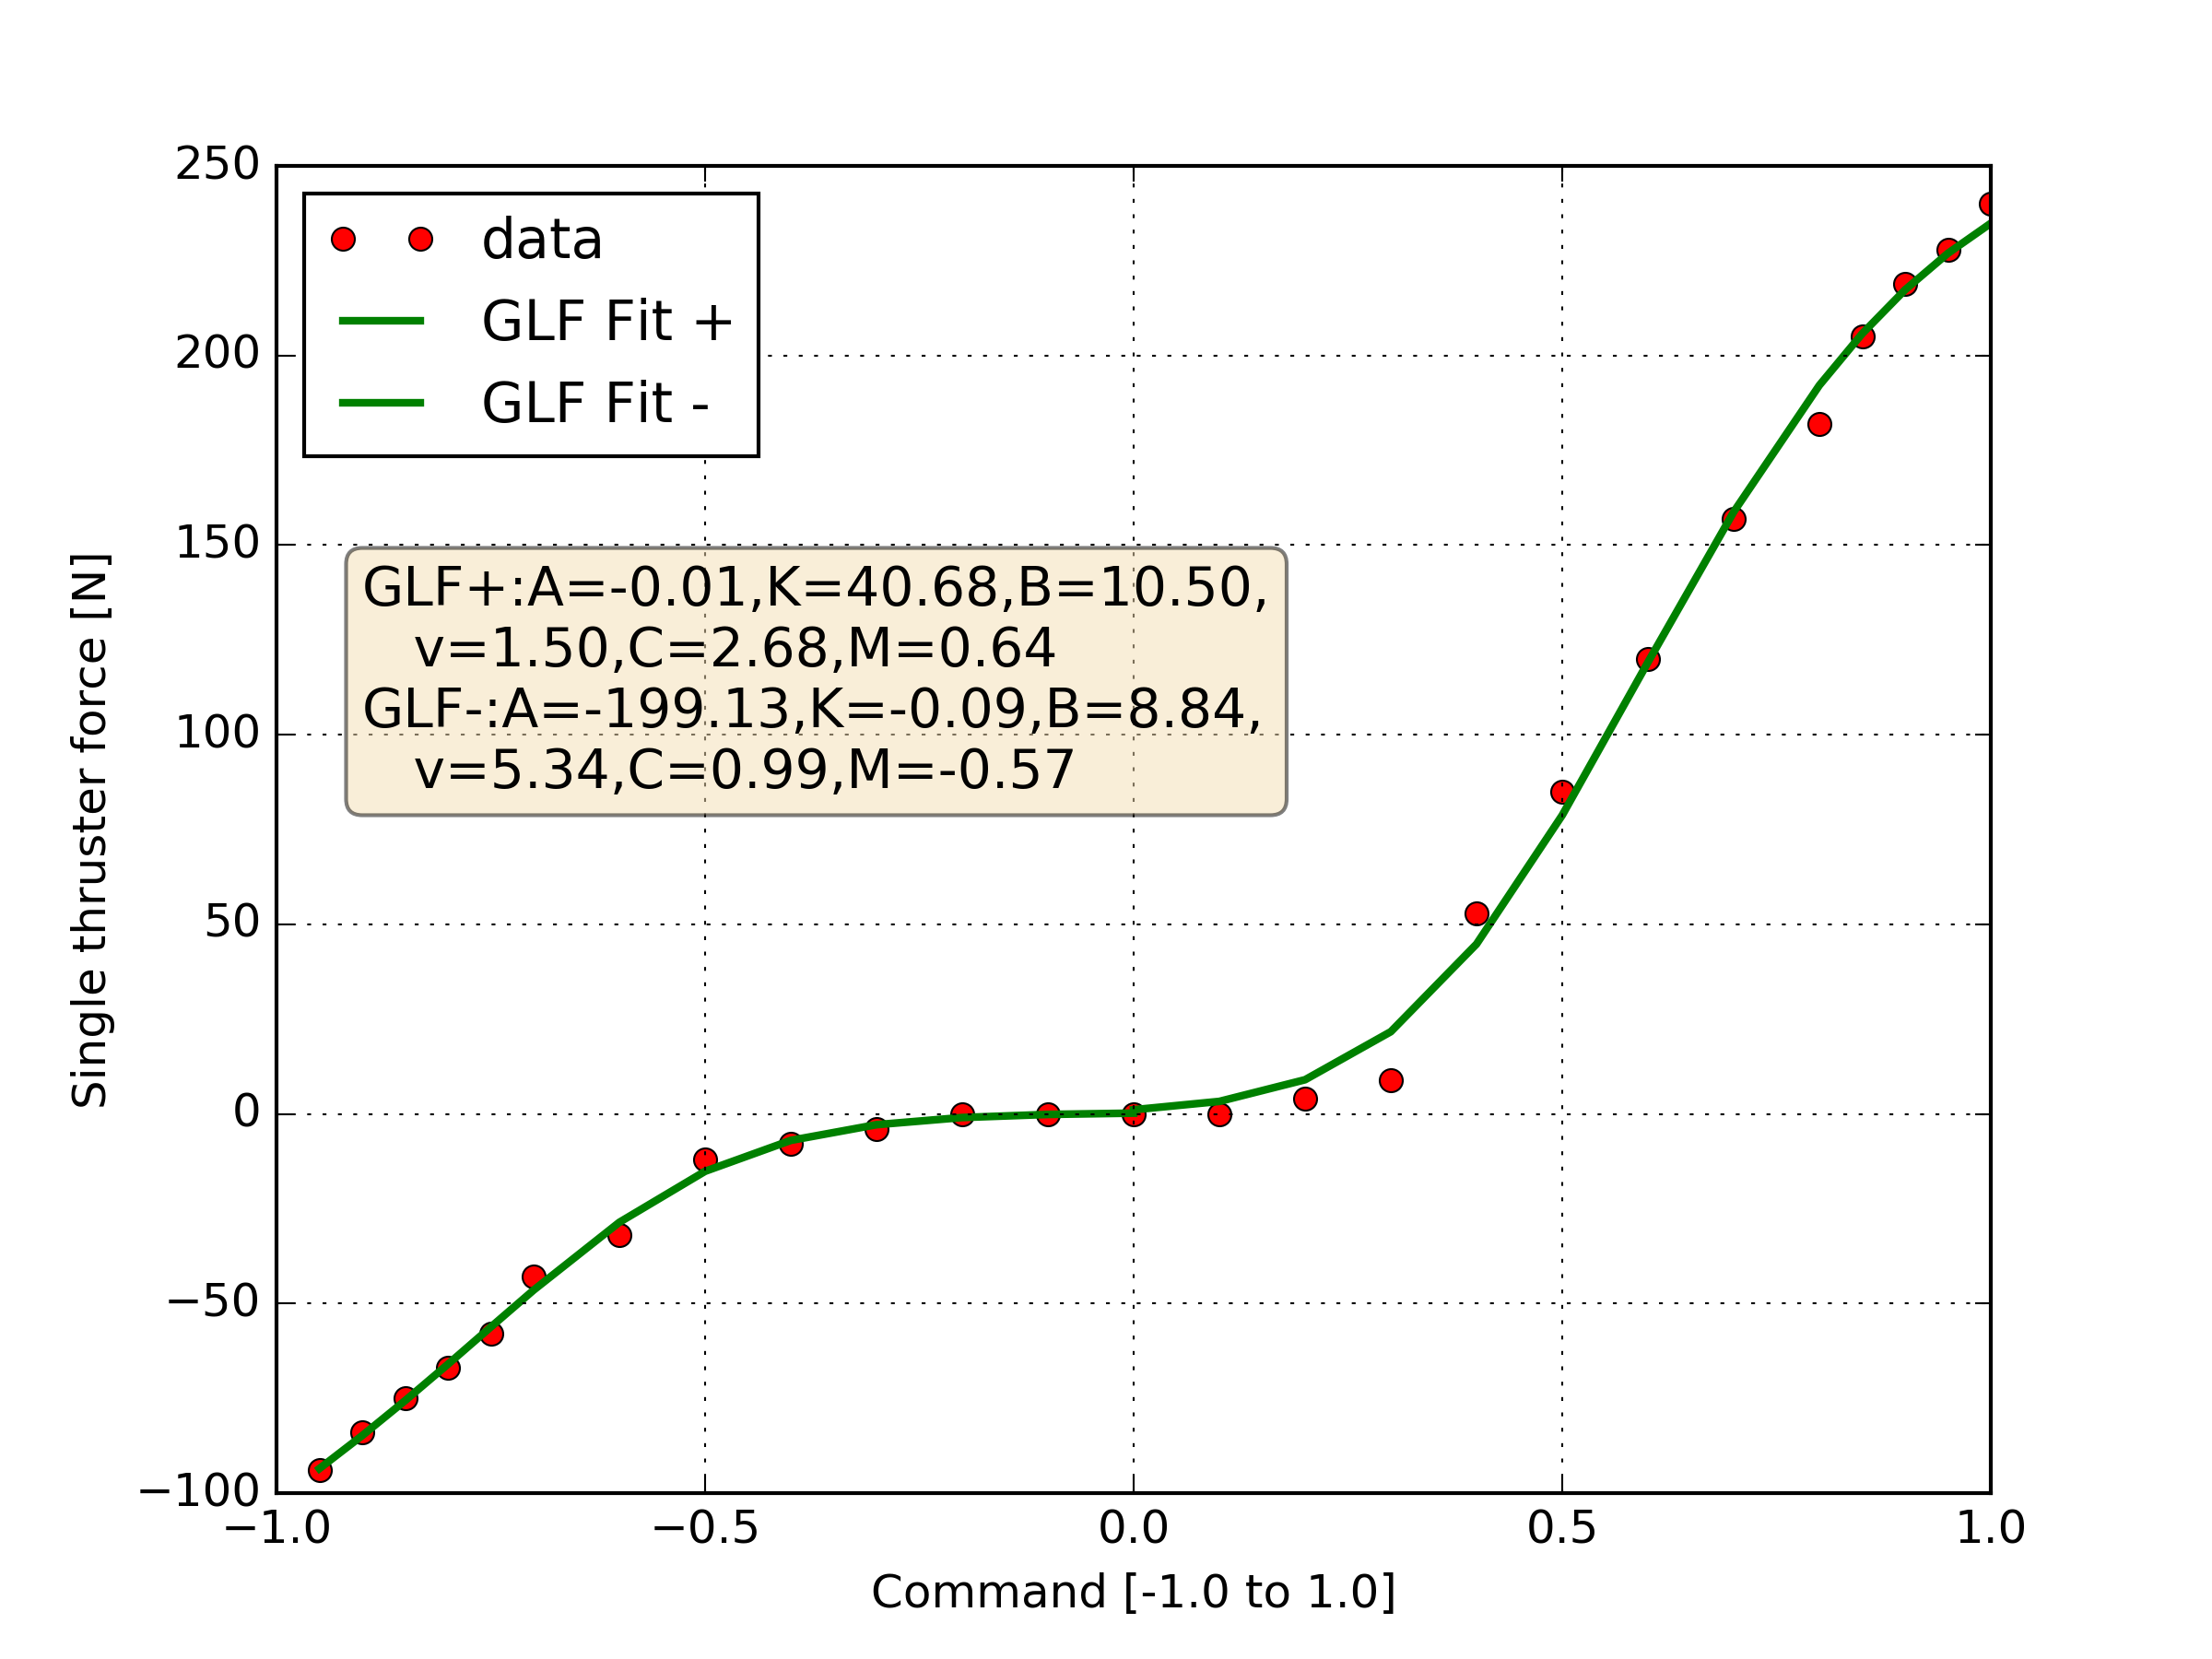
\includegraphics[width=0.6\textwidth]{images/wamv_glf_annote.png}
  \caption{GLF fit of empirical data.}
  \label{f:fit}
\end{figure}


\section{Wind}

The influence of wind on the motion of the USV is implemented as a standalone model plugin for Gazebo.  Currently there is only one implementation, but other implementations, with varying fidelity, could be developed in the future.

\subsection{usv gazebo wind plugin}

The wind forces (x and y) and moment (yaw) are predicted following the models presented by Fossen~\cite{fossen94guidance}.

The wind velocity on the vessel ($V_w$) is considered to be a constant velocity and direction.  If desired, this could be extended to include a parameterized wind spectrum the distribution of wind velocities over time, e.g., average wind velocity, gusts, etc.  For the current implementation the constant wind velocity is specified as a three element vector which specifies the wind speed the world-frame x, y and z coordinates with units of \unitfrac[]{m}{s}.  The z component is ignored.

The resulting forces and moments on the vessel are determined based on the user-specified force/moment coefficients and the relative wind velocity.  Within the plugin, the relative (or apparent) wind velocity vector $V_R$.  The forces/moment are calculated as
\begin{eqnarray}
  X_{wind} &=& (C_X) V_{R_x} |V_{R_x}| \\
  Y_{wind} &=& (C_Y) V_{R_y} |V_{R_y}| \\
  N_{wind} &=& -2.0 (C_N) V_{R_x} V_{R_y} \\
\end{eqnarray}
where $C_X$, $C_Y$ and $C_N$ are specified as the three element \verb+wind_coeff_vector+.  Approximate values for these coefficients are given in \cite{sarda17station} which can then be tuned to give reasonable response.

%\newpage
%\setcounter{page}{1}
\bibliographystyle{ieeetr}
\bibliography{refs}

\end{document}
\grid
